\documentclass[conf]{new-aiaa}
%\documentclass[journal]{new-aiaa} for journal papers
\usepackage[utf8]{inputenc}

\usepackage{graphicx}
\usepackage{amsmath}
\usepackage[version=4]{mhchem}
\usepackage{siunitx}
\usepackage{longtable,tabularx}
\setlength\LTleft{0pt} 

% Two more packages that make it easy to show MATLAB code
\usepackage[T1]{fontenc}
\usepackage[framed,numbered]{matlab-prettifier}
\lstset{
	style = Matlab-editor,
	basicstyle=\mlttfamily\small,
}

% Say where pictures (if any) will be placed
\graphicspath{{./pictures/}}

% Define title, author, and date
\title{AE353: Design Problem 03\\ (Control of Unpowered Glider)}

\author{T. Bretl}


% Start of document
\begin{document}

% Put the title, author, and date at top of first page
\maketitle


\begin{abstract}
This paper describes the third design problem that you will complete in AE353 (Spring 2020). It asks you to design, implement, and test a controller for un unpowered glider, and to submit a report that describes both your method of approach and your results.
\end{abstract}

\section{Nomenclature}

{\renewcommand\arraystretch{1.0}
\noindent\begin{longtable*}{@{}l @{\quad=\quad} l@{}}
$x, y$ & horizontal and vertical position in meters \\
$\dot{x}, \dot{y}$ & horizontal and vertical velocity in meters per second\\
$\theta$ & pitch angle in radians \\
$\dot{\theta}$ & pitch angular rate in radians per second \\
$\phi$ & elevator angle in radians \\
$\dot{\phi}$ & elevator angular rate in radians per second \\
$v$ & airspeed in meters per second \\
$\alpha$ & angle of attack in radians \\
$c_{L}, c_{D}$ & coefficients of lift and drag \\
$\dot{\phi}_{\text{max}}$ & maximum elevator angular rate in radians per second
\end{longtable*}}



\section{Goal}

The code provided in \lstinline!DesignProblem03! simulates an unpowered glider that is similar to one used for experiments on fixed-wing perching \cite{Roberts2009,Moore2014}. This glider has one control surface, an elevator. An actuator allows you to specify the angular rate of this elevator. Sensors allow you to measure both the pitch angle and the airspeed of the glider. The goal is to make the glider fly as long a distance as possible, as reliably as possible, if released at a height of about two meters with a forward speed of about six meters per second and with a pitch angle of your choice.

\section{Model}

The motion of the glider is governed by ordinary differential equations with the form
\begin{equation}
\label{eqEOM}
\begin{bmatrix} \ddot{x} \\ \ddot{y} \\ \ddot{\theta} \end{bmatrix} = f(\theta,\phi,\dot{x},\dot{y},\dot{\theta},\dot{\phi})
\end{equation}
where $\theta$ is the pitch angle, $\phi$ is the elevator angle, $\dot{x}$ is the forward speed, $\dot{y}$ is the vertical speed, $\dot{\theta}$ is the pitch angular rate, and $\dot{\phi}\in[-\dot{\phi}_\text{max}, \dot{\phi}_\text{max}]$ is the elevator angular rate (which an actuator allows you to specify). You might be interested to know that these equations were derived by applying a flat-plate model of lift $c_{L}$ and drag $c_{D}$ as a function of angle of attack $\alpha$, for both the wing and elevator:
\begin{equation*}
c_{L} = 2\sin\alpha \cos\alpha
\qquad\qquad
c_{D} = 2\sin^{2}\alpha
\end{equation*}
Experimental results show that this flat-plate model is a good approximation for the glider and that it remains accurate at high angles of attack and even post-stall \cite{Moore2014}. The function $f$ in \eqref{eqEOM} depends on a number of parameters (e.g., mass, moment of inertia, surface area of the wing). You can save both a symbolic description and a numeric description of this function to a file for later analysis if you call the simulator with the optional parameter \lstinline|'eomfile'|, for example as follows:
\begin{quote}
\begin{lstlisting}
% Run the simulator to save the equations of motion
DesignProblem03('Controller', 'eomfile', 'eom.mat', 'display', 'false');
% Load the equations of motion
load('eom.mat');
% Parse the equations of motion
f = symEOM.f;
% Define symbolic variables that appear in the equations of motion
syms theta phi xdot ydot thetadot phidot
% Proceed to linearize or do whatever else you like...
% 	(see: help sym/jacobian, help sym/diff, help sym/subs, etc.)
\end{lstlisting}
\end{quote}
Assuming zero wind, the airspeed sensor measures the component of velocity that is aligned with the wing:
\[
\text{airspeed} = \dot{x} \cos\theta + \dot{y} \sin\theta
\]
This sensor cannot measure ``negative airspeed,'' so if $\text{airspeed} < 0$ then the sensor will produce a zero measurement.




\section{Tasks}


\subsection{Analysis}
\label{secAnalysis}

The focus of your analysis this time will be on data collection. The initial conditions in the simulation are random. So, for a given control design, the flight distance will vary (perhaps significantly). It is not enough to look at the results of one flight---you will have to look at the results of many flights. At minimum, for each design and for each launch angle that you consider, you should do the following:
\begin{itemize}
\item Collect data from at least 1000 flights.
\item Compute the minimum, maximum, median, mean, and standard deviation of the flight distance (e.g., \lstinline|min|, \lstinline|max|, \lstinline|median|, \lstinline|mean|, and \lstinline|std| in MATLAB).
\item Plot a histogram of the flight distance (e.g., \lstinline|hist| in MATLAB).
\end{itemize}
Remember that \lstinline|DesignProblem03| provides options to save data and to turn the graphics off, both of which are useful for data collection. Here is an example of how to use these options to collect and analyze data from many flights.
\begin{quote}
\begin{lstlisting}
% Number of flights
nFlights = 1e3;
% Loop over each flight
for i=1:nFlights
    % Run simulation without graphics and save data
    DesignProblem03('Controller','datafile','data.mat','display',false);
    % Load data
    load('data.mat');
    % Get t and x
    t = processdata.t;
    x = processdata.x;
    % Do analysis...
    %     (your code here)
end
\end{lstlisting}
\end{quote}


\subsection{Presentation}

The focus of your presentation this time will be on equations. For example, you should be sure to do the following:
\begin{itemize}
\item Number any equation to which you will refer, and do the reference with \lstinline|\eqref|.
\item Use standard notation for operations like multiplication (e.g., $Ax$ for ``$A$ times $x$'' and not $A\times x$ or $A*x$).
\item Place square brackets around matrices. For example,
\begin{quote}
\begin{lstlisting}[language={[LaTeX]TeX}]
\begin{bmatrix} \ddot{x} \\ \ddot{y} \\ \ddot{\theta} \end{bmatrix}
\end{lstlisting}
\end{quote}
produces the standard notation
\begin{equation*}
\begin{bmatrix} \ddot{x} \\ \ddot{y} \\ \ddot{\theta} \end{bmatrix},
\end{equation*}
while
\begin{quote}
\begin{lstlisting}[language={[LaTeX]TeX}]
\begin{matrix} \ddot{x} \\ \ddot{y} \\ \ddot{\theta} \end{matrix}
\end{lstlisting}
\end{quote}
produces the non-standard and confusing notation
\begin{equation*}
\begin{matrix} \ddot{x} \\ \ddot{y} \\ \ddot{\theta} \end{matrix}.
\end{equation*}
\item Align equations properly. For example,
\begin{quote}
\begin{lstlisting}[language={[LaTeX]TeX}]
\begin{align*}
c_{L} &= 2\sin\alpha \cos\alpha \\ 
c_{D} &= 2\sin^{2}\alpha
\end{align*}
\end{lstlisting}
\end{quote}
produces the nice-looking result
\begin{align*}
c_{L} &= 2\sin\alpha \cos\alpha \\ 
c_{D} &= 2\sin^{2}\alpha
\end{align*}
while
\begin{quote}
\begin{lstlisting}[language={[LaTeX]TeX}]
\begin{equation*}
c_{L} = 2\sin\alpha \cos\alpha
\end{equation*}
\begin{equation*}
c_{D} = 2\sin^{2}\alpha
\end{equation*}
\end{lstlisting}
\end{quote}
produces the messy-looking result
\begin{equation*}
c_{L} = 2\sin\alpha \cos\alpha
\end{equation*}
\begin{equation*}
c_{D} = 2\sin^{2}\alpha.
\end{equation*}
\item Use the correct font for functions like cosine (\lstinline|$\cos\alpha$| produces a nice-looking $\cos\alpha$, while \lstinline|$cos\alpha$| produces a messy-looking $cos\alpha$).
\end{itemize}
Please be responsive to feedback on your draft reports---this feedback will focus on helping you improve your presentation of equations.

\subsection{Report}
\label{report}

Your report must be a PDF document that was generated using \LaTeX\ and that conforms to the guidelines for ``Preparation of Papers for AIAA Technical Conferences'' (\url{https://go.aerospace.illinois.edu/aiaa-latex-template}). The author must be listed as ``Anonymous'' (with no affiliations). The report must be exactly four pages. It must have the following sections:
\begin{itemize}
\item {\em Abstract}. Summarize your key results in one short paragraph.
\item {\em Nomenclature}. List all symbols used in your report, with units.
\item {\em Goal}. At minimum, this section will describe the system you have been asked to control, define one requirement and one verification (which must depend on rigorous data collection and analysis as described in Section \ref{secAnalysis}), and prepare the reader to understand the rest of your report.
\item {\em Model.} At minimum, this section will linearize \eqref{eqEOM} about some choice of equilibrium point, expressing the result in state-space form.
\item {\em Control Design.} At minimum, this section will present the design of a controller and an observer (remembering to check, first, that the linearized model is both controllable and observable).
\item {\em Results.} At minimum, this section will describe what you did to implement and test your controller and observer in simulation. It will show that you have followed the instructions that you wrote to verify that your requirement has (or has not) been satisfied and will, in particular, include at least one figure of aggregate results (e.g., a histogram). It will also include at least one figure that provides evidence the observer is working (e.g., a plot of the error in the state estimate as a function of time).
\end{itemize}
You are encouraged to go beyond these minimum requirements. For example, it is likely that you will want to iterate on your design and on your choice of initial launch angle, in order to maximize flight distance. In this case, it would be helpful to describe the process that you used to improve your design.


\section{Deliverables}

\subsection{Submit a first draft by 11:59PM on Wednesday, April 1, 2020}
\label{secDraft01}

This draft must be a PDF document that follows the guidelines provided in Section \ref{report} and that includes, at minimum, a {\bf complete draft} of your ``Goal'' and ``Model'' sections. It must be submitted here:
\begin{quote}
\url{https://forms.illinois.edu/sec/3018672}
\end{quote}
You may submit as many times as you want---only the last submission will be recorded.

\subsection{Submit a second draft by 11:59PM on Monday, April 6, 2020}
\label{secDraft02}

This draft must be a PDF document that follows the guidelines provided in Section \ref{report} and that includes, at minimum, a {\bf complete draft} of your ``Control Design'' and ``Results'' sections. It must be submitted here:
\begin{quote}
\url{https://forms.illinois.edu/sec/7635612}
\end{quote}
You may submit as many times as you want---only the last submission will be recorded.

\subsection{Submit a final report by 11:59PM on Friday, April 10, 2020}

This report must be a PDF document that follows the guidelines provided in Section \ref{report}. You must submit three things in addition to the report:
\begin{itemize}
\item The \LaTeX\ source files that you used to produce the document (in a ZIP folder with all figures, references, etc., in addition to the \lstinline|.tex| file). Please do {\em not} include MATLAB code with your \LaTeX\ source files.
\item The MATLAB code that you used to produce all of the figures, tables, and other results that are included in the document (in a ZIP folder). Your code must have a MATLAB script called \lstinline|GenerateResults.m|. It should be possible for any of your peers to reproduce {\em everything} in your report by executing this script. Please do {\em not} include \LaTeX\ source files with your MATLAB code.
\item The implementation of your ``best'' controller as a single file \lstinline|Controller.m|. If one of your peers runs the simulator with this controller, they should see behavior that is consistent with claims made in the report.
\end{itemize}
Your report must be submitted here:
\begin{quote}
\url{https://forms.illinois.edu/sec/1071483}
\end{quote}
You may submit as many times as you want---only the last submission will be recorded.


\section{Evaluation}

Your work will be evaluated based on meeting intermediate deadlines (20\%) and on staff reviews of your code (20\%) and of your report (60\%).

Reviews of your technical approach will place special emphasis on {\em data collection and analysis}. Reviews of your report will place special emphasis on your {\em presentation of equations}.

Staff review will be ``double-blind.'' You won't know who reviewed your report, and your reviewers won't know whose report they reviewed. To enable a double-blind review process, it is \textbf{very important} that your final report be completely anonymous. To repeat, \textbf{DO NOT INCLUDE YOUR NAME} or anything else that would identify you in any of the materials you submit---not in your PDF, in your two ZIP folders, or in your MATLAB script.


\section{On-Time Submission}

Draft reports and final reports must be submitted on time or they will receive zero credit. I am so serious about this that I will even give you extra credit if you submit your final report early:
\begin{quote}
\textbf{If the last submission of your final report occurs by 11:59PM on Wednesday, April 8, 2020---so, 48 hours before the final deadline---then you will receive 5\% extra credit.}
\end{quote}
Please do not put yourself in the danger zone (Figure \ref{figSubTimes}). An easy way to make sure you do not receive zero credit is to submit each of your first two drafts (Sections \ref{secDraft01}-\ref{secDraft02}), as soon as you write them, also as your final report.

\begin{figure}[h!]
\begin{center}
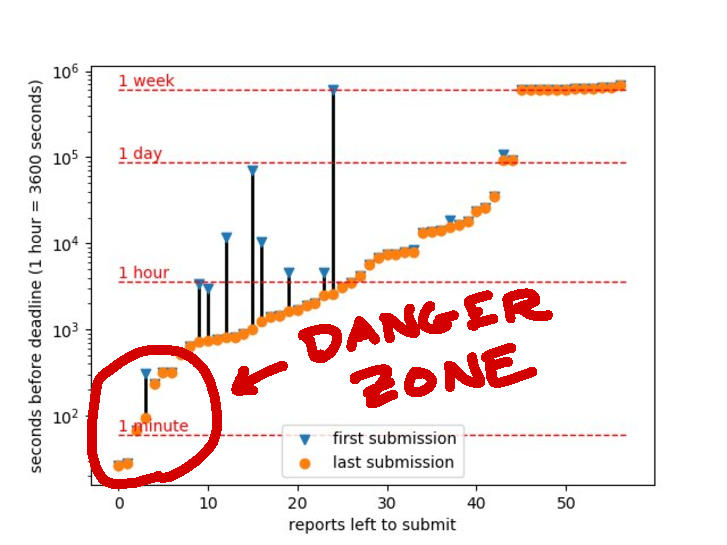
\includegraphics[width=0.6\textwidth]{submission_times_DP02}
\caption{Submission times for the second design report this semester. If you choose to submit your final report for the first time at the last minute, you are asking for trouble.}
\label{figSubTimes}
\end{center}
\end{figure}



% Display list of references in IEEE Transactions format.
\bibliographystyle{IEEEtran}
\bibliography{IEEEabrv,references}

% End of document (everything after this is ignored)
\end{document}